\documentclass[border=8pt]{standalone}
\usepackage{tikz}
\usetikzlibrary{arrows.meta, decorations.pathreplacing}
\colorlet{pvcol}{red!70!black}
\colorlet{sstcol}{green!45!black}
\colorlet{vipcol}{orange!85!black}
\colorlet{ngfcol}{violet!70!black}
\begin{document}
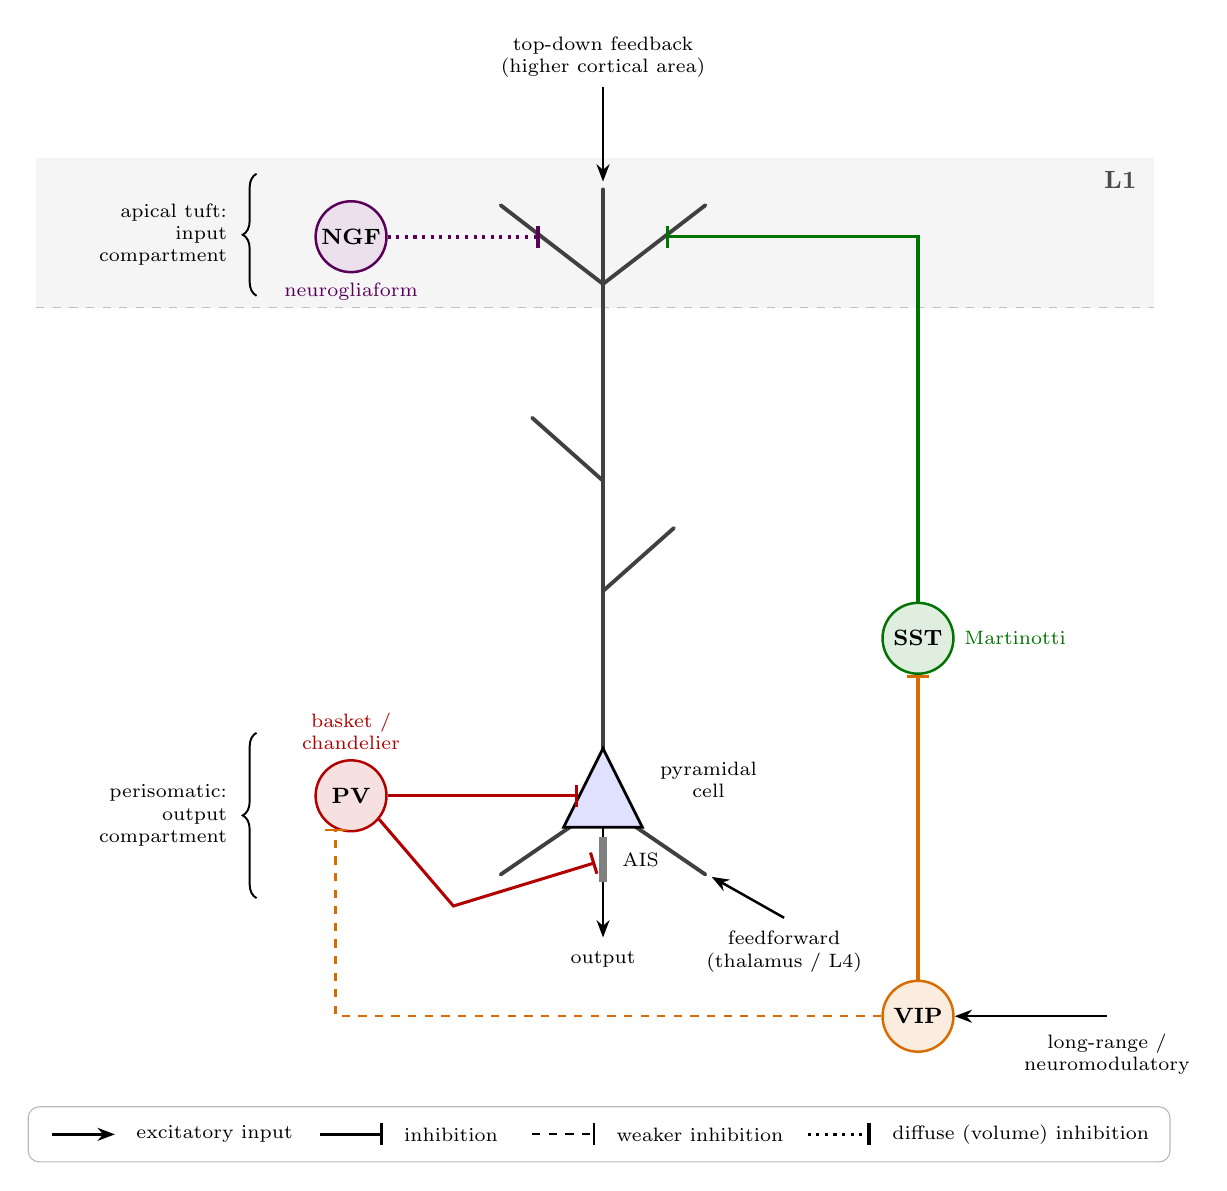
\begin{tikzpicture}[
  font=\footnotesize,
  dend/.style={line width=1.4pt, draw=black!75, line cap=round},
  exc/.style={-{Stealth[length=2.2mm]}, line width=0.9pt},
  inh/.style={-{Bar[width=2.8mm]}, line width=1.1pt},
  weak/.style={inh, dashed, line width=0.8pt},
  diffuse/.style={inh, dotted, line width=1.3pt},
  cell/.style={circle, draw, line width=0.9pt, minimum size=9mm, inner sep=0pt,
               font=\footnotesize\bfseries},
  lbl/.style={font=\scriptsize, align=center},
]
  % ---- Layer 1 band ----
  \fill[gray!8] (-7.2,6.6) rectangle (7.0,8.5);
  \draw[gray!50, dashed] (-7.2,6.6) -- (7.0,6.6);
  \node[anchor=north east, font=\small\bfseries, text=gray!60!black] at (6.9,8.45) {L1};

  % ---- Pyramidal cell ----
  \draw[dend] (0,1.0) -- (0,6.9);                  % apical trunk
  \draw[dend] (0,3.0) -- (0.9,3.8);                % oblique dendrites
  \draw[dend] (0,4.4) -- (-0.9,5.2);
  \draw[dend] (0,6.9) -- (-1.3,7.9);               % apical tuft in L1
  \draw[dend] (0,6.9) -- (0,8.1);
  \draw[dend] (0,6.9) -- (1.3,7.9);
  \draw[dend] (-0.35,0.05) -- (-1.3,-0.6);         % basal dendrites
  \draw[dend] (0.35,0.05) -- (1.3,-0.6);
  \draw[exc] (0,0) -- (0,-1.4);                    % axon (output)
  \draw[line width=3pt, black!50] (0,-0.12) -- (0,-0.7);   % axon initial segment
  \filldraw[fill=blue!12, draw=black, line width=1pt] (-0.5,0) -- (0.5,0) -- (0,1.0) -- cycle;
  \node[lbl, anchor=west] at (0.6,0.6) {pyramidal\\cell};
  \node[lbl, anchor=west] at (0.12,-0.42) {AIS};
  \node[lbl, anchor=north] at (0,-1.45) {output};

  % ---- Interneurons ----
  \node[cell, draw=pvcol,  fill=pvcol!12]  (pv)  at (-3.2,0.4) {PV};
  \node[cell, draw=sstcol, fill=sstcol!12] (sst) at (4.0,2.4)  {SST};
  \node[cell, draw=vipcol, fill=vipcol!12] (vip) at (4.0,-2.4) {VIP};
  \node[cell, draw=ngfcol, fill=ngfcol!12] (ngf) at (-3.2,7.5) {NGF};
  \node[lbl, anchor=south, text=pvcol]  at (pv.north)  {basket /\\chandelier};
  \node[lbl, anchor=west,  text=sstcol] at (sst.east)  {Martinotti};
  \node[lbl, anchor=north, text=ngfcol] at (ngf.south) {neurogliaform};

  % ---- Inhibitory connections ----
  \draw[inh, pvcol]      (pv.east) -- (-0.32,0.4);                     % PV basket -> soma
  \draw[inh, pvcol]      (pv.-40) -- (-1.9,-1.0) -- (-0.1,-0.45);      % PV chandelier -> AIS
  \draw[inh, sstcol]     (sst.north) -- (4.0,7.5) -- (0.8,7.5);        % SST -> apical tuft
  \draw[inh, vipcol]     (vip.north) -- (sst.south);                   % VIP -> SST
  \draw[weak, vipcol]    (vip.west) -| (pv.-115);                      % VIP -> PV (weaker)
  \draw[diffuse, ngfcol] (ngf.east) -- (-0.8,7.5);                     % NGF -> tuft (volume)

  % ---- Excitatory inputs ----
  \draw[exc] (0,9.4) -- (0,8.2);
  \node[lbl, anchor=south] at (0,9.4) {top-down feedback\\(higher cortical area)};
  \draw[exc] (2.3,-1.15) -- (1.38,-0.63);
  \node[lbl, anchor=north] at (2.3,-1.2) {feedforward\\(thalamus / L4)};
    \draw[exc] (6.4,-2.4) -- (vip.east);
  \node[lbl, anchor=north] at (6.4,-2.5) {long-range /\\neuromodulatory};

  % ---- Compartment braces ----
  \draw[decorate, decoration={brace, amplitude=5pt}, line width=0.7pt]
      (-4.4,-0.9) -- (-4.4,1.2)
      node[midway, left=7pt, lbl, align=right] {perisomatic:\\output\\compartment};
  \draw[decorate, decoration={brace, amplitude=5pt}, line width=0.7pt]
      (-4.4,6.75) -- (-4.4,8.3)
      node[midway, left=7pt, lbl, align=right] {apical tuft:\\input\\compartment};

  % ---- Legend ----
    \begin{scope}[shift={(-7.0,-3.9)}]
    \draw[exc]     (0,0)   -- (0.8,0);  \node[lbl, anchor=west] at (0.95,0)  {excitatory input};
    \draw[inh]     (3.4,0) -- (4.2,0);  \node[lbl, anchor=west] at (4.35,0)  {inhibition};
    \draw[weak]    (6.1,0) -- (6.9,0);  \node[lbl, anchor=west] at (7.05,0)  {weaker inhibition};
    \draw[diffuse] (9.6,0) -- (10.4,0); \node[lbl, anchor=west] at (10.55,0) {diffuse (volume) inhibition};
    \draw[gray!55, rounded corners=4pt] (-0.3,0.35) rectangle (14.2,-0.35);
  \end{scope}
\end{tikzpicture}
\end{document}